
\serie{Egalité de vecteurs}

\begin{exercice}
On considère un parallélogramme} ABCD, dont les diagonales se coupent en O.

\begin{enumerate}
\item Pour chacune des questions suivantes, compléter par un vecteur égal.

\begin{multicols}{2}[\raggedcolumns]
\begin{enumerate}%[label=(\alph*)]
\item $\overrightarrow{AB}=\hdots\hdots$
\item $\overrightarrow{BC}=\hdots\hdots$
\item $\overrightarrow{DO}=\hdots\hdots$
\item $\overrightarrow{OA}=\hdots\hdots$
\item $\overrightarrow{CD}=\hdots\hdots$
\end{enumerate}
\end{multicols}

\item Pour chacune des affirmations suivantes, dire si elle est vraie ou fausse, en justifiant.

\begin{multicols}{2}[\raggedcolumns]
\begin{enumerate}%[label=(\alph*)]
\item $\overrightarrow{OB}=\overrightarrow{OC}$
\item $[$AB$]=[$DC$]$
\item $\overrightarrow{OA}=\overrightarrow{OC}$
\item AB $=$ DC
\item $\overrightarrow{AA}=\overrightarrow{BB}$
\end{enumerate}
\end{multicols}
\end{enumerate}

\end{exercice}


\begin{exercice}

On considère les points A, B, C, D, E et F placés sur le quadrillage ci-dessous.

\vspace{0.25cm}
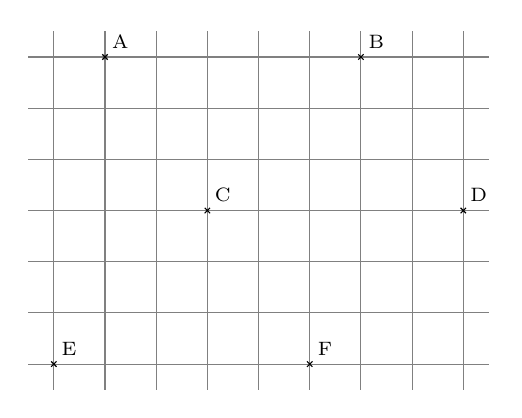
\begin{tikzpicture}[scale=0.65]
\draw [color=gray, xstep=1,ystep=1] (-0.5,-0.5) grid (8.5,6.5);
\begin{scriptsize}
\draw [color=black] (0.,0.)-- ++(-1.5pt,-1.5pt) -- ++(3.0pt,3.0pt) ++(-3.0pt,0) -- ++(3.0pt,-3.0pt);
\draw[color=black] (0.3,0.3) node {E};
\draw [color=black] (5.,0.)-- ++(-1.5pt,-1.5pt) -- ++(3.0pt,3.0pt) ++(-3.0pt,0) -- ++(3.0pt,-3.0pt);
\draw[color=black] (5.3,0.3) node {F};
\draw [color=black] (3.,3.)-- ++(-1.5pt,-1.5pt) -- ++(3.0pt,3.0pt) ++(-3.0pt,0) -- ++(3.0pt,-3.0pt);
\draw[color=black] (3.3,3.3) node {C};
\draw [color=black] (8.,3.)-- ++(-1.5pt,-1.5pt) -- ++(3.0pt,3.0pt) ++(-3.0pt,0) -- ++(3.0pt,-3.0pt);
\draw[color=black] (8.3,3.3) node {D};
\draw [color=black] (6.,6.)-- ++(-1.5pt,-1.5pt) -- ++(3.0pt,3.0pt) ++(-3.0pt,0) -- ++(3.0pt,-3.0pt);
\draw[color=black] (6.3,6.3) node {B};
\draw [color=black] (1.,6.)-- ++(-1.5pt,-1.5pt) -- ++(3.0pt,3.0pt) ++(-3.0pt,0) -- ++(3.0pt,-3.0pt);
\draw[color=black] (1.3,6.3) node {A};
\end{scriptsize}
\end{tikzpicture}}

Dire si chacune des égalités suivantes est vraie ou fausse.

\begin{multicols}{2}[\raggedcolumns]
\begin{enumerate}%[label=(\alph*)]
\item $\overrightarrow{AB}=\overrightarrow{EF}$
\item $\overrightarrow{CD}=-\overrightarrow{AB}$
\item $\overrightarrow{DA}=\overrightarrow{DB}$
\item $\overrightarrow{ED}=\overrightarrow{BD}$
\item $\overrightarrow{AE}=\overrightarrow{BF}$
\item $\overrightarrow{EF}=-\overrightarrow{DC}$
\end{enumerate}
\end{multicols}
\end{exercice}


\begin{exercice}

On considère la figure ci-dessous, formée de parallélogrammes juxtaposés.

\vspace{0.25cm}
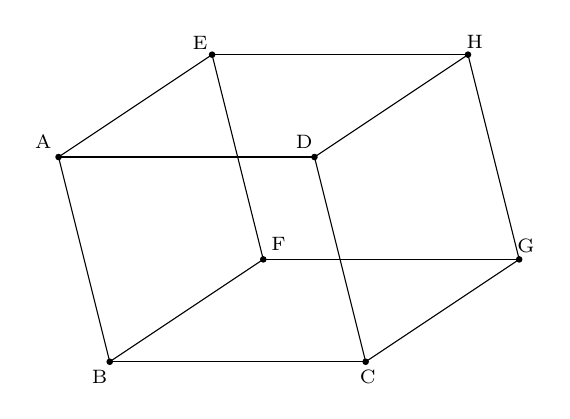
\begin{tikzpicture}[scale=0.65]
\draw (0.,4.)-- (1.,0.);
\draw (1.,0.)-- (6.,0.);
\draw (6.,0.)-- (9.,2.);
\draw (9.,2.)-- (8.,6.);
\draw (8.,6.)-- (3.,6.);
\draw (3.,6.)-- (0.,4.);
\draw (0.,4.)-- (5.,4.);
\draw (5.,4.)-- (6.,0.);
\draw (3.,6.)-- (4.,2.);
\draw (4.,2.)-- (9.,2.);
\draw (1.,0.)-- (4.,2.);
\draw (5.,4.)-- (8.,6.);
\begin{scriptsize}
\draw [fill=black] (0.,4.) circle (1.5pt);
\draw[color=black] (-0.3,4.3) node {A};
\draw [fill=black] (1.,0.) circle (1.5pt);
\draw[color=black] (0.8,-0.3) node {B};
\draw [fill=black] (6.,0.) circle (1.5pt);
\draw[color=black] (6.04,-0.3) node {C};
\draw [fill=black] (5.,4.) circle (1.5pt);
\draw[color=black] (4.8,4.3) node {D};
\draw [fill=black] (3.,6.) circle (1.5pt);
\draw[color=black] (2.767272727272728,6.2363636363636346) node {E};
\draw [fill=black] (4.,2.) circle (1.5pt);
\draw[color=black] (4.3,2.3) node {F};
\draw [fill=black] (9.,2.) circle (1.5pt);
\draw[color=black] (9.13090909090909,2.254545454545456) node {G};
\draw [fill=black] (8.,6.) circle (1.5pt);
\draw[color=black] (8.13090909090909,6.254545454545453) node {H};
\end{scriptsize}
\end{tikzpicture}

Déterminer un représentant de :

\begin{multicols}{2}[\raggedcolumns]
\begin{enumerate}%[label=(\alph*)]
\item $\overrightarrow{AE}$ ;
\item $\overrightarrow{DB}$ ;
\item $\overrightarrow{FG}$ d'origine B ;
\item $\overrightarrow{CF}$ d'extrémité E ;
\item $\overrightarrow{0}$ ;
\item $-\overrightarrow{AF}$.
\end{enumerate}
\end{multicols}

\end{exercice}

\begin{exercice}
Soit ABCD et CDEF deux parallélogrammes.\\

Montrer que ABFE est aussi un parallélogramme.
\end{exercice}

\begin{exercice}
ABCD est un rectangle de centre O.
\begin{enumerate}
\item Démontrer que $\overrightarrow{AO}=\overrightarrow{OC}$
\item Compléter en utilisant les points de la figure:
\begin{description}
\item $\overrightarrow{BO}= . . . $;
\item $\overrightarrow{CO}= . . . $;
\item $\overrightarrow{DO}= . . . $.
\end{description}
\end{enumerate}
\end{exercice}

\serie{Construction de vecteurs}

\begin{exercice}
Soit ABC un triangle quelconque.

\begin{enumerate}
\item Construire :

\begin{itemize}
\item le point N tel que $\overrightarrow{AN}=\overrightarrow{BC}$ ;
\item le point P tel que $\overrightarrow{PA}=\overrightarrow{BC}$ ;
\item le point M tel que $\overrightarrow{BM}=\overrightarrow{AC}$.
\end{itemize}

\item Montrer que A, B et C sont les milieux respectifs de $[$NP$]$, $[$PM$]$ et $[$MN$]$.

\end{enumerate}
\end{exercice}

\begin{exercice}
\begin{minipage}{0.27\linewidth}
On considère le parallélogramme ABCD représenté ci-contre.
\end{minipage}
\hspace{0.25cm}
\begin{minipage}{0.6\linewidth}
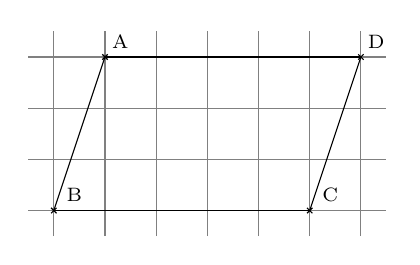
\begin{tikzpicture}[scale=0.65]
\draw [color=gray, xstep=1,ystep=1] (-0.5,-0.5) grid (6.5,3.5);
\begin{scriptsize}
\draw [color=black] (0.,0.)-- ++(-1.5pt,-1.5pt) -- ++(3.0pt,3.0pt) ++(-3.0pt,0) -- ++(3.0pt,-3.0pt);
\draw[color=black] (0.4,0.3) node {B};
\draw [color=black] (5.,0.)-- ++(-1.5pt,-1.5pt) -- ++(3.0pt,3.0pt) ++(-3.0pt,0) -- ++(3.0pt,-3.0pt);
\draw[color=black] (5.4,0.3) node {C};
\draw [color=black] (1.,3.)-- ++(-1.5pt,-1.5pt) -- ++(3.0pt,3.0pt) ++(-3.0pt,0) -- ++(3.0pt,-3.0pt);
\draw[color=black] (1.3,3.3) node {A};
\draw [color=black] (6.,3.)-- ++(-1.5pt,-1.5pt) -- ++(3.0pt,3.0pt) ++(-3.0pt,0) -- ++(3.0pt,-3.0pt);
\draw[color=black] (6.3,3.3) node {D};
\end{scriptsize}
\draw (0,0) -- (5,0);
\draw (1,3) -- (6,3);
\draw (0,0) -- (1,3);
\draw (5,0) -- (6,3);
\end{tikzpicture}
\end{minipage}

\begin{enumerate}%[label=(\alph*)]
\item Reproduire le parallélogramme ABCD sur un quadrillage.
\item Construire les points E, F, G, H et I définis par :

\begin{multicols}{2}[\raggedcolumns]
\begin{itemize}
\item $\overrightarrow{CE}=\overrightarrow{AC}$ ;
\item $\overrightarrow{CF}=\overrightarrow{AB}$ ;
\item $\overrightarrow{EG}=\overrightarrow{CD}$ ;
\item $\overrightarrow{AH}=-\overrightarrow{BC}$ ;
\item $\overrightarrow{IA}=\overrightarrow{AC}$ ;
\end{itemize}
\end{multicols}
\item Quelle est la nature des quadrilatères BCEF et DGEC ? Justifier.
\item Que représente le point A pour le segment $[$IC$]$ ? Justifier.
\end{enumerate}
\end{exercice}

\begin{exercice}
Soit ABCD un parallélogramme quelconque.
\begin{enumerate}
\item Construire le point N tel que $\overrightarrow{AN}=\overrightarrow{CB}$;
\item Que représente le point A pour le segment [DN]? Justifier;
\item Construire le point P tel que $\overrightarrow{PA}=\overrightarrow{DC}$;
\item Construire le point M tel que $\overrightarrow{BM}=\overrightarrow{AC}$;
\item Quel est la nature du quadrilatère ABMC?Justifier.
\end{enumerate}
\end{exercice}


%%%%%%%%%%%%%%%%%%%%%%%%%%%%%%%%%%%%%%%%%%%%%%%%%%%

\serie{Opérations sur les vecteurs}

\begin{exercice}
On considère la figure ci-dessous :

\vspace{0.25cm}
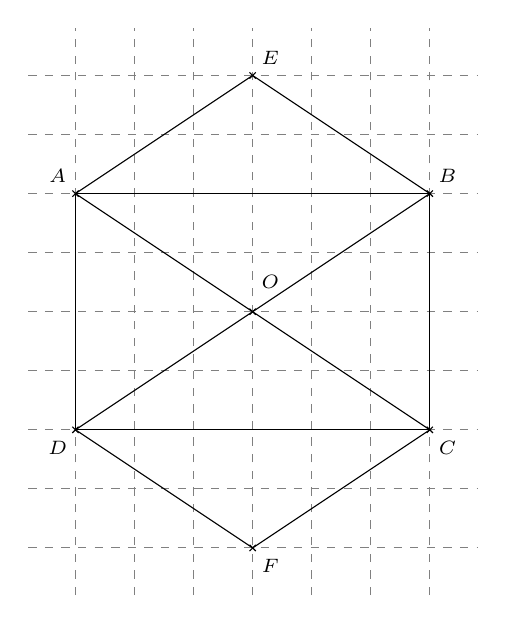
\begin{tikzpicture}[scale=0.75]
\draw [color=gray,dash pattern=on 3pt off 3pt,xstep=1,ystep=1] (-0.8,-2.8) grid (6.8,6.8);
\draw (0.,4.)-- (0.,0.);
\draw (0.,0.)-- (6.,0.);
\draw (6.,0.)-- (6.,4.);
\draw (6.,4.)-- (0.,4.);
\draw (0.,4.)-- (3.,6.);
\draw (3.,6.)-- (6.,4.);
\draw (6.,0.)-- (3.,-2.);
\draw (3.,-2.)-- (0.,0.);
\draw (0.,0.)-- (6.,4.);
\draw (0.,4.)-- (6.,0.);
\begin{scriptsize}
\draw [color=black] (0.,0.)-- ++(-1.5pt,-1.5pt) -- ++(3.0pt,3.0pt) ++(-3.0pt,0) -- ++(3.0pt,-3.0pt);
\draw[color=black] (-0.3,-0.3) node {$D$};
\draw [color=black] (6.,0.)-- ++(-1.5pt,-1.5pt) -- ++(3.0pt,3.0pt) ++(-3.0pt,0) -- ++(3.0pt,-3.0pt);
\draw[color=black] (6.3,-0.3) node {$C$};
\draw [color=black] (6.,4.)-- ++(-1.5pt,-1.5pt) -- ++(3.0pt,3.0pt) ++(-3.0pt,0) -- ++(3.0pt,-3.0pt);
\draw[color=black] (6.3,4.3) node {$B$};
\draw [color=black] (0.,4.)-- ++(-1.5pt,-1.5pt) -- ++(3.0pt,3.0pt) ++(-3.0pt,0) -- ++(3.0pt,-3.0pt);
\draw[color=black] (-0.3,4.3) node {$A$};
\draw [color=black] (3.,6.)-- ++(-1.5pt,-1.5pt) -- ++(3.0pt,3.0pt) ++(-3.0pt,0) -- ++(3.0pt,-3.0pt);
\draw[color=black] (3.3,6.3) node {$E$};
\draw [color=black] (3.,-2.)-- ++(-1.5pt,-1.5pt) -- ++(3.0pt,3.0pt) ++(-3.0pt,0) -- ++(3.0pt,-3.0pt);
\draw[color=black] (3.3,-2.3) node {$F$};
\draw [color=black] (3.,2.)-- ++(-1.5pt,-1.5pt) -- ++(3.0pt,3.0pt) ++(-3.0pt,0) -- ++(3.0pt,-3.0pt);
\draw[color=black] (3.3,2.5) node {$O$};
\end{scriptsize}
\end{tikzpicture}

\vspace{0.25cm}
Donner dans chaque cas un représentant de la somme ou de la différence des vecteurs :

\vspace{0.25cm}
\begin{itemize}
\item $\overrightarrow{AE}+\overrightarrow{AO}$ ;
\item $\overrightarrow{AE}+\overrightarrow{DF}$ ;
\item $\overrightarrow{OC}-\overrightarrow{FC}$ ;
\item $\overrightarrow{DO}+\overrightarrow{BC}+\overrightarrow{AE}$ ;
\item $\overrightarrow{BD}-\overrightarrow{BA}$.
\end{itemize}
\end{exercice}


\begin{exercice}
On considère la figure ci-dessous, formée de parallélogrammes juxtaposés.

\vspace{0.25cm}
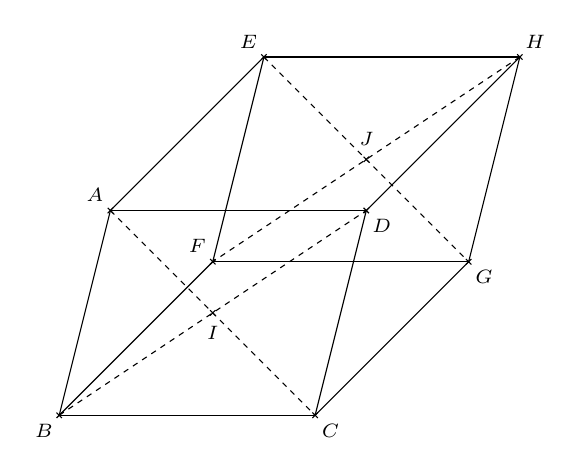
\begin{tikzpicture}[scale=0.65]
\draw (0.,0.)-- (1.,4.);
\draw (1.,4.)-- (6.,4.);
\draw (6.,4.)-- (5.,0.);
\draw (5.,0.)-- (0.,0.);
\draw [dash pattern=on 2pt off 2pt] (1.,4.)-- (5.,0.);
\draw [dash pattern=on 2pt off 2pt] (0.,0.)-- (6.,4.);
\draw (0.,0.)-- (3.,3.);
\draw (3.,3.)-- (8.,3.);
\draw (8.,3.)-- (9.,7.);
\draw (9.,7.)-- (4.,7.);
\draw (4.,7.)-- (3.,3.);
\draw [dash pattern=on 2pt off 2pt] (4.,7.)-- (8.,3.);
\draw [dash pattern=on 2pt off 2pt] (9.,7.)-- (3.,3.);
\draw (1.,4.)-- (4.,7.);
\draw (6.,4.)-- (9.,7.);
\draw (5.,0.)-- (8.,3.);
\begin{scriptsize}
\draw [color=black] (0.,0.)-- ++(-1.5pt,-1.5pt) -- ++(3.0pt,3.0pt) ++(-3.0pt,0) -- ++(3.0pt,-3.0pt);
\draw[color=black] (-0.3,-0.3) node {$B$};
\draw [color=black] (1.,4.)-- ++(-1.5pt,-1.5pt) -- ++(3.0pt,3.0pt) ++(-3.0pt,0) -- ++(3.0pt,-3.0pt);
\draw[color=black] (0.7,4.3) node {$A$};
\draw [color=black] (6.,4.)-- ++(-1.5pt,-1.5pt) -- ++(3.0pt,3.0pt) ++(-3.0pt,0) -- ++(3.0pt,-3.0pt);
\draw[color=black] (6.3,3.7) node {$D$};
\draw [color=black] (5.,0.)-- ++(-1.5pt,-1.5pt) -- ++(3.0pt,3.0pt) ++(-3.0pt,0) -- ++(3.0pt,-3.0pt);
\draw[color=black] (5.3,-0.3) node {$C$};
\draw [color=black] (3.,3.)-- ++(-1.5pt,-1.5pt) -- ++(3.0pt,3.0pt) ++(-3.0pt,0) -- ++(3.0pt,-3.0pt);
\draw[color=black] (2.7,3.3) node {$F$};
\draw [color=black] (4.,7.)-- ++(-1.5pt,-1.5pt) -- ++(3.0pt,3.0pt) ++(-3.0pt,0) -- ++(3.0pt,-3.0pt);
\draw[color=black] (3.7,7.3) node {$E$};
\draw [color=black] (9.,7.)-- ++(-1.5pt,-1.5pt) -- ++(3.0pt,3.0pt) ++(-3.0pt,0) -- ++(3.0pt,-3.0pt);
\draw[color=black] (9.3,7.3) node {$H$};
\draw [color=black] (8.,3.)-- ++(-1.5pt,-1.5pt) -- ++(3.0pt,3.0pt) ++(-3.0pt,0) -- ++(3.0pt,-3.0pt);
\draw[color=black] (8.3,2.7) node {$G$};
\draw [color=black] (3.,2.)-- ++(-1.5pt,-1.5pt) -- ++(3.0pt,3.0pt) ++(-3.0pt,0) -- ++(3.0pt,-3.0pt);
\draw[color=black] (3,1.6) node {$I$};
\draw [color=black] (6.,5.)-- ++(-1.5pt,-1.5pt) -- ++(3.0pt,3.0pt) ++(-3.0pt,0) -- ++(3.0pt,-3.0pt);
\draw[color=black] (6,5.4) node {$J$};
\end{scriptsize}
\end{tikzpicture}

\vspace{0.25cm}
Déterminer un représentant de :

\begin{multicols}{2}[\raggedcolumns]
\begin{enumerate}%[label=(\alph*)]
\item $\overrightarrow{AD}+\overrightarrow{CF}$ ;
\item $\overrightarrow{GC}+\overrightarrow{AC}$ ;
\item $\overrightarrow{HE}+\overrightarrow{BC}$ ;
\item $\overrightarrow{DE}-\overrightarrow{DH}$ ;
\item $\overrightarrow{GJ}+\overrightarrow{BF}$ ;
\item $\overrightarrow{IF}-\overrightarrow{FJ}$ ;
\item $\overrightarrow{AF}+\overrightarrow{HD}+\overrightarrow{BD}$ ;
\item $\overrightarrow{JE}+\overrightarrow{FG}-\overrightarrow{ID}$.
\end{enumerate}
\end{multicols}
\end{exercice} 


\begin{exercice}
Dans chacun des cas, construire le vecteur d’origine A égal à la somme $\overrightarrow{u}+\overrightarrow{v}$:

\begin{center}
\definecolor{yqyqyq}{rgb}{0.501960784314,0.501960784314,0.501960784314}
\begin{tikzpicture}[line cap=round,line join=round,>=triangle 45,x=1.0cm,y=1.0cm]
\draw [color=yqyqyq,dash pattern=on 4pt off 4pt, xstep=1.0cm,ystep=1.0cm] (-2.87,-0.51) grid (5.23,6.63);
\clip(-2.87,-0.51) rectangle (5.23,6.63);
\draw [->] (-2.,1.) -- (1.,5.);
\draw [->] (1.,5.) -- (4.,2.);
\begin{scriptsize}
\draw [color=black] (-2.,1.)-- ++(-1.5pt,-1.5pt) -- ++(3.0pt,3.0pt) ++(-3.0pt,0) -- ++(3.0pt,-3.0pt);
\draw[color=black] (-2.3,1.5) node {$A$};
\draw[color=black] (-0.59,3.57) node {$\overrightarrow{u}$};
\draw[color=black] (2.65,3.84) node {$\overrightarrow{v}$};
\end{scriptsize}
\end{tikzpicture}
\end{center}}
\begin{center}
\definecolor{yqyqyq}{rgb}{0.501960784314,0.501960784314,0.501960784314}
\begin{tikzpicture}[line cap=round,line join=round,>=triangle 45,x=1.0cm,y=1.0cm]
\draw [color=yqyqyq,dash pattern=on 4pt off 4pt, xstep=1.0cm,ystep=1.0cm] (-2.87,-0.51) grid (5.23,6.63);
\clip(-2.87,-0.51) rectangle (5.23,6.63);
\draw [->] (-1.,3.) -- (1.,5.);
\draw [->] (2.,6.) -- (4.,5.);
\begin{scriptsize}
\draw [color=black] (-2.,1.)-- ++(-1.5pt,-1.5pt) -- ++(3.0pt,3.0pt) ++(-3.0pt,0) -- ++(3.0pt,-3.0pt);
\draw[color=black] (-2.3,1.5) node {$A$};
\draw[color=black] (-0.26,4.32) node {$\overrightarrow{u}$};
\draw[color=black] (3.22,5.82) node {$\overrightarrow{v}$};
\end{scriptsize}
\end{tikzpicture}
\end{center}
\begin{center}
\definecolor{yqyqyq}{rgb}{0.501960784314,0.501960784314,0.501960784314}
\begin{tikzpicture}[line cap=round,line join=round,>=triangle 45,x=1.0cm,y=1.0cm]
\draw [color=yqyqyq,dash pattern=on 4pt off 4pt, xstep=1.0cm,ystep=1.0cm] (-3.77,-3.09) grid (3.19,4.05);
\clip(-3.77,-3.09) rectangle (3.19,4.05);
\draw [->] (-2.,-1.) -- (0.,-2.);
\draw [->] (2.,0.) -- (0.,-2.);
\begin{scriptsize}
\draw [color=black] (-2.,2.)-- ++(-1.5pt,-1.5pt) -- ++(3.0pt,3.0pt) ++(-3.0pt,0) -- ++(3.0pt,-3.0pt);
\draw[color=black] (-2.3,2.52) node {$A$};
\draw[color=black] (-0.89,-1.14) node {$\overrightarrow{u}$};
\draw[color=black] (0.9,-0.81) node {$\overrightarrow{v}$};
\end{scriptsize}
\end{tikzpicture}
\end{center}
\end{exercice} 

\begin{exercice}
Sur chacune des figures suivantes, construire un représentant de $\overrightarrowc{u}+\overrightarrowc{v}$ :

\begin{enumerate}
\item \ \

\begin{tikzpicture}[scale=0.75]
\draw [-latex] (0.,0.) -- (4.,1.);
\draw [-latex] (0.,0.) -- (-2.,3.);
\begin{scriptsize}
\draw [color=black,thick] (0.,0.)-- ++(-2pt,-2pt) -- ++(4pt,4pt) ++(-4pt,0) -- ++(4pt,-4pt);
\draw (2,0.5) node[below] {$\overrightarrowc{u}$};
\draw (-1,1.7) node[above] {$\overrightarrowc{v}$};
\draw [color=white] (-3,5) circle (1pt);
\draw [color=white] (0,-2) circle (1pt);
\end{scriptsize}
\end{tikzpicture}

\item \ \

\begin{tikzpicture}[scale=0.75]
\draw [-latex] (0.,0.) -- (5.,-1.);
\draw [-latex] (0.,0.) -- (-2.,0.4);
\begin{scriptsize}
\draw [color=black,thick] (0.,0.)-- ++(-2pt,-2pt) -- ++(4pt,4pt) ++(-4pt,0) -- ++(4pt,-4pt);
\draw (-1,0.2) node[above] {$\overrightarrowc{u}$};
\draw (2.5,-0.5) node[below] {$\overrightarrowc{v}$};
\draw [color=white] (-3,2.5) circle (1pt);
\draw [color=white] (0,-2.5) circle (1pt);
\end{scriptsize}
\end{tikzpicture}

\item \ \

\begin{tikzpicture}[scale=0.75]
\draw [-latex] (0.,0.) -- (2.,4.);
\draw [-latex] (-2.,-1.) -- (3.,-2.);
\begin{scriptsize}
\draw [color=black,thick] (0.,0.)-- ++(-2pt,-2pt) -- ++(4pt,4pt) ++(-4pt,0) -- ++(4pt,-4pt);
\draw [color=black,thick] (-2,-1)-- ++(-2pt,-2pt) -- ++(4pt,4pt) ++(-4pt,0) -- ++(4pt,-4pt);
\draw (0.8,2) node[above] {$\overrightarrowc{u}$};
\draw (0.5,-1.5) node[below] {$\overrightarrowc{v}$};
\draw [color=white] (-3,3) circle (1pt);
\draw [color=white] (0,-4) circle (1pt);
\end{scriptsize}
\end{tikzpicture}

\item \ \

\begin{tikzpicture}[scale=0.75]
\draw [-latex] (0.,0.) -- (-4.,1.);
\draw [-latex] (2.,2.) -- (-4.,1.);
\begin{scriptsize}
\draw [color=black,thick] (0.,0.)-- ++(-2pt,-2pt) -- ++(4pt,4pt) ++(-4pt,0) -- ++(4pt,-4pt);
\draw [color=black,thick] (2,2)-- ++(-2pt,-2pt) -- ++(4pt,4pt) ++(-4pt,0) -- ++(4pt,-4pt);
\draw (-2,0.5) node[below] {$\overrightarrowc{u}$};
\draw (-1,1.5) node[above] {$\overrightarrowc{v}$};
\draw [color=white] (-7,5) circle (1pt);
\draw [color=white] (0,-2) circle (1pt);
\end{scriptsize}
\end{tikzpicture}
\end{enumerate}
\end{exercice} 

\begin{exercice}
En utilisant la relation de Chasles, simplifier au maximum les vecteurs suivants :

\begin{enumerate}

\item $\overrightarrow{u}=\overrightarrow{AB}+\overrightarrow{BC}+\overrightarrow{CE}+\overrightarrow{EG}$
 
\item $\overrightarrow{w}=\overrightarrow{AB}+\overrightarrow{CB}+\overrightarrow{BD}+\overrightarrow{DE}$

\item $\overrightarrow{v}=\overrightarrow{AB}+\overrightarrow{DA}+\overrightarrow{CD}+\overrightarrow{BC}$ 

\item $\overrightarrow{n}=\overrightarrow{AG}+\overrightarrow{DE}+\overrightarrow{CD}+\overrightarrow{GC}$
\end{enumerate}
\end{exercice} 

\begin{exercice}
Simplifier au maximun les vecteurs suivants:
\begin{enumerate}
\item $\overrightarrow{AB}+\overrightarrow{BC}+\overrightarrow{CA}$;
\item $\overrightarrow{IJ}+\overrightarrow{KI}+\overrightarrow{JK}$;
\item $\overrightarrow{DE}+\overrightarrow{FG}+\overrightarrow{EF}-\overrightarrow{DG}$.
\end{enumerate}
\end{exercice}

\begin{exercice}
Sur chacune des figures suivantes, construire un représentant de $\overrightarrowc{u}-\overrightarrowc{v}$ :

\begin{enumerate}
\item \ \

\begin{tikzpicture}[scale=0.75]
\draw [-latex] (0.,0.) -- (4.,1.);
\draw [-latex] (0.,0.) -- (-2.,3.);
\begin{scriptsize}
\draw [color=black,thick] (0.,0.)-- ++(-2pt,-2pt) -- ++(4pt,4pt) ++(-4pt,0) -- ++(4pt,-4pt);
\draw (2,0.5) node[below] {$\overrightarrowc{u}$};
\draw (-1,1.7) node[above] {$\overrightarrowc{v}$};
\draw [color=white] (-3,5) circle (1pt);
\draw [color=white] (0,-2) circle (1pt);
\end{scriptsize}
\end{tikzpicture}

\item \ \

\begin{tikzpicture}[scale=0.75]
\draw [-latex] (0.,0.) -- (5.,-1.);
\draw [-latex] (0.,0.) -- (-2.,0.4);
\begin{scriptsize}
\draw [color=black,thick] (0.,0.)-- ++(-2pt,-2pt) -- ++(4pt,4pt) ++(-4pt,0) -- ++(4pt,-4pt);
\draw (-1,0.2) node[above] {$\overrightarrowc{u}$};
\draw (2.5,-0.5) node[below] {$\overrightarrowc{v}$};
\draw [color=white] (-3,2.5) circle (1pt);
\draw [color=white] (0,-2.5) circle (1pt);
\end{scriptsize}
\end{tikzpicture}

\item \ \

\begin{tikzpicture}[scale=0.75]
\draw [-latex] (0.,0.) -- (2.,4.);
\draw [-latex] (-2.,-1.) -- (3.,-2.);
\begin{scriptsize}
\draw [color=black,thick] (0.,0.)-- ++(-2pt,-2pt) -- ++(4pt,4pt) ++(-4pt,0) -- ++(4pt,-4pt);
\draw [color=black,thick] (-2,-1)-- ++(-2pt,-2pt) -- ++(4pt,4pt) ++(-4pt,0) -- ++(4pt,-4pt);
\draw (0.8,2) node[above] {$\overrightarrowc{u}$};
\draw (0.5,-1.5) node[below] {$\overrightarrowc{v}$};
\draw [color=white] (-3,3) circle (1pt);
\draw [color=white] (0,-4) circle (1pt);
\end{scriptsize}
\end{tikzpicture}

\item \ \

\begin{tikzpicture}[scale=0.75]
\draw [-latex] (0.,0.) -- (-4.,1.);
\draw [-latex] (2.,2.) -- (-4.,1.);
\begin{scriptsize}
\draw [color=black,thick] (0.,0.)-- ++(-2pt,-2pt) -- ++(4pt,4pt) ++(-4pt,0) -- ++(4pt,-4pt);
\draw [color=black,thick] (2,2)-- ++(-2pt,-2pt) -- ++(4pt,4pt) ++(-4pt,0) -- ++(4pt,-4pt);
\draw (-2,0.5) node[below] {$\overrightarrowc{u}$};
\draw (-1,1.5) node[above] {$\overrightarrowc{v}$};
\draw [color=white] (-7,5) circle (1pt);
\draw [color=white] (0,-2) circle (1pt);
\end{scriptsize}
\end{tikzpicture}
\end{enumerate}
\end{exercice} 

\begin{exercice}
Reproduire chacune des figures suivantes, puis construire le vecteur demandé :

\vspace{0.25cm}
\renewcommand{\arraystretch}{0.6}
\begin{tabular}{m{0.2cm}ll}
1. & \ 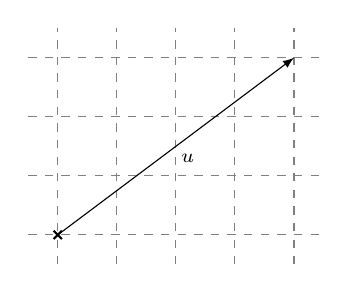
\begin{tikzpicture}[scale=0.75]
\draw [color=gray,dash pattern=on 3pt off 3pt,xstep=1,ystep=1] (-0.5,-0.5) grid (4.5,3.5);
\draw [-latex] (0,0) -- (4,3);
\begin{scriptsize}
\draw [color=black,thick] (0.,0.)-- ++(-2pt,-2pt) -- ++(4pt,4pt) ++(-4pt,0) -- ++(4pt,-4pt);
\draw (2.2,1.5) node[below] {$\overrightarrowc{u}$};
\end{scriptsize}
\end{tikzpicture}
& $2,5\overrightarrowc{u}$ ;\\
&&\\
2. & \ 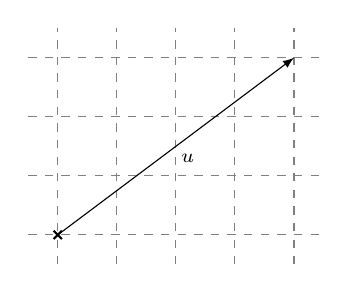
\begin{tikzpicture}[scale=0.75]
\draw [color=gray,dash pattern=on 3pt off 3pt,xstep=1,ystep=1] (-0.5,-0.5) grid (4.5,3.5);
\draw [-latex] (0,0) -- (4,3);
\begin{scriptsize}
\draw [color=black,thick] (0.,0.)-- ++(-2pt,-2pt) -- ++(4pt,4pt) ++(-4pt,0) -- ++(4pt,-4pt);
\draw (2.2,1.5) node[below] {$\overrightarrowc{u}$};
\end{scriptsize}
\end{tikzpicture}
& $-\dfrac{3}{4}\overrightarrowc{u}$ ;\\
&&\\
3. & \ 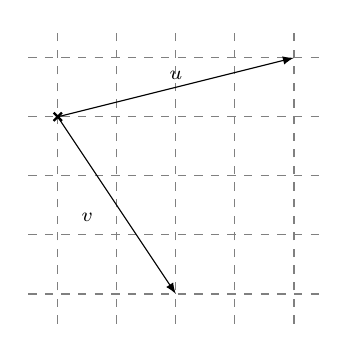
\begin{tikzpicture}[scale=0.75]
\draw [color=gray,dash pattern=on 3pt off 3pt,xstep=1,ystep=1] (-0.5,-1.5) grid (4.5,3.5);
\draw [-latex] (0,2) -- (4,3);
\draw [-latex] (0,2) -- (2,-1);
\draw [color=black,thick] (0,2)-- ++(-2pt,-2pt) -- ++(4pt,4pt) ++(-4pt,0) -- ++(4pt,-4pt);
\begin{scriptsize}
\draw (2,2.5) node[above] {$\overrightarrowc{u}$};
\draw (0.5,0.5) node[below] {$\overrightarrowc{v}$};
\end{scriptsize}
\end{tikzpicture}
& $3\overrightarrowc{u}-2\overrightarrowc{v}$ ;\\
&&\\
4. & \ 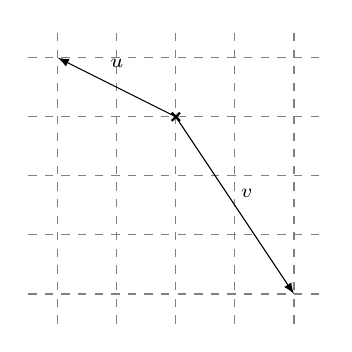
\begin{tikzpicture}[scale=0.75]
\draw [color=gray,dash pattern=on 3pt off 3pt,xstep=1,ystep=1] (-0.5,-1.5) grid (4.5,3.5);
\draw [-latex] (2,2) -- (0,3);
\draw [-latex] (2,2) -- (4,-1);
\draw [color=black,thick] (2,2)-- ++(-2pt,-2pt) -- ++(4pt,4pt) ++(-4pt,0) -- ++(4pt,-4pt);
\begin{scriptsize}
\draw (1,2.7) node[above] {$\overrightarrowc{u}$};
\draw (3.2,0.5) node[above] {$\overrightarrowc{v}$};
\end{scriptsize}
\end{tikzpicture}
& $-\dfrac{5}{2}\overrightarrowc{u}+\dfrac{2}{3}\overrightarrowc{v}$ ;\\
\end{tabular}
\end{exercice} 

\begin{exercice}
Construire le vecteur d’origine A égale à $3\overrightarrow{u}+2\overrightarrow{v}$.

\begin{tikzpicture}[line cap=round,line join=round,>=triangle 45,x=1.0cm,y=1.0cm]
\clip(-3.77,-2.7) rectangle (5.2,4.95);
\draw [->] (-2.,-1.) -- (0.,-2.);
\draw [->] (1.18,-2.19) -- (2.44,-1.14);
\begin{scriptsize}
\draw [color=black] (-2.,3.)-- ++(-1.5pt,-1.5pt) -- ++(3.0pt,3.0pt) ++(-3.0pt,0) -- ++(3.0pt,-3.0pt);
\draw[color=black] (-2.3,3.51) node {$A$};
\draw[color=black] (-0.89,-1.14) node {$\overrightarrow{u}$};
\draw[color=black] (1.57,-1.32) node {$\overrightarrow{v}$};
\end{scriptsize}
\end{tikzpicture}
\end{exercice} 

\begin{exercice}
Construire le vecteur d’origine A égale à $\overrightarrow{u}-2\overrightarrow{v}$.

\begin{tikzpicture}[line cap=round,line join=round,>=triangle 45,x=1.0cm,y=1.0cm]
\clip(-4.82,-2.73) rectangle (4.15,4.92);
\draw [->] (-2.,-1.) -- (0.,-2.);
\draw [->] (1.18,-2.19) -- (2.44,-1.14);
\begin{scriptsize}
\draw [color=black] (-2.,3.)-- ++(-1.5pt,-1.5pt) -- ++(3.0pt,3.0pt) ++(-3.0pt,0) -- ++(3.0pt,-3.0pt);
\draw[color=black] (-2.3,3.51) node {$A$};
\draw[color=black] (-0.89,-1.14) node {$\overrightarrow{u}$};
\draw[color=black] (1.57,-1.32) node {$\overrightarrow{v}$};
\end{scriptsize}
\end{tikzpicture}
\end{exercice}

\begin{exercice}
Construire les points M, N, et P définis par : $\overrightarrow{AM}=\dfrac{2}{3}\overrightarrow{u}$; $\overrightarrow{AN}=-2\overrightarrow{v}$  et $\overrightarrow{BP}=-\dfrac{1}{3}\overrightarrow{u}+\overrightarrow{v}$ .\\

\definecolor{yqyqyq}{rgb}{0.501960784314,0.501960784314,0.501960784314}
\begin{tikzpicture}[line cap=round,line join=round,>=triangle 45,x=1.0cm,y=1.0cm]
\draw [color=yqyqyq,dash pattern=on 4pt off 4pt, xstep=1.0cm,ystep=1.0cm] (-5.84,-0.93) grid (2.62,6.72);
\clip(-5.84,-0.93) rectangle (2.62,6.72);
\draw [->] (-5.,3.) -- (-2.,6.);
\draw [->] (0.,0.) -- (-2.,1.);
\begin{scriptsize}
\draw [color=black] (-2.,3.)-- ++(-1.5pt,-1.5pt) -- ++(3.0pt,3.0pt) ++(-3.0pt,0) -- ++(3.0pt,-3.0pt);
\draw[color=black] (-2.3,3.51) node {$A$};
\draw[color=black] (-3.65,4.86) node {$\overrightarrow{u}$};
\draw[color=black] (-0.74,0.78) node {$\overrightarrow{v}$};
\draw [color=black] (1.,5.)-- ++(-1.5pt,-1.5pt) -- ++(3.0pt,3.0pt) ++(-3.0pt,0) -- ++(3.0pt,-3.0pt);
\draw[color=black] (1.21,5.43) node {$B$};
\end{scriptsize}
\end{tikzpicture}
\end{exercice}

\begin{exercice}
Simplifier au maximun les vecteurs suivants:
\begin{enumerate}
\item $\overrightarrow{AE}+\overrightarrow{FT}+\overrightarrow{KA}+\overrightarrow{EF}$ ;
\item $\overrightarrow{AB}-\overrightarrow{AC}-\overrightarrow{CB}$ ;
\item $\overrightarrow{AC}+2\overrightarrow{CB}+\overrightarrow{BA}$ ;
\item $-\overrightarrow{HD}+\overrightarrow{ZA}+\overrightarrow{HR}-\overrightarrow{DN}+\overrightarrow{RZ}$ ;
\item $3\overrightarrow{AB}+2\overrightarrow{BC}+4\overrightarrow{CA}$ ;
\item $\overrightarrow{AB}-2\overrightarrow{AC}+2\overrightarrow{BC}$.
\end{enumerate}
\end{exercice}






